\documentclass[
	A4paper,
	DIV=9,
	BCOR7mm,
	smallheadings,
	headinclude,
	footinclude,
	headsepline,
	parindent,
	german,
	captions=tableheading,
	abstracton
	]{scrreprt}
\usepackage{blindtext}
\usepackage[ngerman]{babel}
\usepackage[T1]{fontenc}
\usepackage[utf8]{inputenc}
\usepackage{lmodern}
\usepackage{microtype}
\usepackage{geometry}
\geometry{
	left=2.5cm,
	right=2cm,
	top=2cm,
	bottom=3cm
	}
\usepackage{float}
\usepackage{graphicx}
\usepackage{tabularx}
\usepackage{enumitem}
\usepackage{amssymb}
\usepackage{xcolor}
\usepackage{hyperref}
\hypersetup{
		colorlinks	= true,
		linkcolor	= blue,
		urlcolor	= blue,
		citecolor	= blue,
		pdftitle    = {},
  		pdfsubject  = {},
  		pdfauthor   = {Panagiota Sismanidou},
  		pdfkeywords = {} ,
  		pdfcreator  = {pdflatex},
  		pdfproducer = {LaTeX with hyperref}
	}
\usepackage{biblatex}
\bibliography{Literaturverzeichnis}


\title{Enterprise Architecture Management}
\author{Panagiota Sismanidou}
\date{30.08.2018}

\begin{document}
\maketitle
\tableofcontents

%\listoffigures
%\listoftables



\chapter{Einführung in Enterprise Architecture Management}

Bis zu vorherigem Zeitpunkt erforderten Computermanipulationsverfahren keine derart ausgefeilten Managementstrategien. Heute implementieren Unternehmen neue Technologien, um die Struktur von Unternehmen zu organisieren und einen strategischen Vorteil zu erlangen, weil diese Verfahren im Laufe der Zeit immer komplexer werden.

In der ersten Phase der Business-Integration und IT (ab Mitte der 80er Jahre bis Mitte der 90er Jahre) war es unmöglich, die Automatisierung von Geschäftsprozessen zu realisieren, die auch in der Vor-Computer-Ära existierte. Die zweite Phase (von Mitte der 1990er bis Mitte der 2000er Jahre) ist die Neuorganisation von Geschäftsprozessen. Es wurde davon ausgegangen, dass die Architekten des Informationssystems eine neue Geschäftsorganisationsstruktur anbieten würden, die mit der IT so kompatibel wie möglich ist. Dieser Zeitraum fiel mit der Begeisterung für ERP-Systeme und Geschäftsprozessmodellierungswerkzeuge zusammen. In diesem Zeitraum, in den neue Produkte und Anwendungen  nehmen Platz auf dem Markt, steigen die Anforderungen an die Anpassungsfähigkeit von Unternehmen jedes Jahr. Es besteht die Notwendigkeit für viele makroökonomische Indikatoren zu einer noch umfassenderen Konsolidierung der verschiedenen  Bereiche eines Unternehmens oder einer Organisation durch den Einsatz elektronischer Werkzeuge.

\section{Enterprise Architecture Management Definition}
Als eine Lösung für das Problem der Anpassungsfähigkeit neuer Technologien in der Struktur eines Unternehmens ist das Enterprise Architecture Management (EAM). EnterpriseArchitecture Management hilft dabei, alle Funktionen innerhalb der Organisation zu synchronisieren und initiiert gleichzeitig einen Zyklus kontinuierlicher Änderungen für die Zwecke der Geschäftsoptimierung. Es gibt keine einheitliche Definition in der Literatur, denn jeder Autor beschreibt die Bedeutung des EAM anders. Eine sehr hilfreiche Definition die ausführlich die Beschreibung des EAM dokumentiert ist folgende:

\begin{quote}Enterprise Architecture Management (EAM) ist ein systematischer und ganzheitlicher Ansatz für das Verstehen, Kommunizieren, Gestalten und Planen der fachlichen und technischen Strukturen im Unternehmen. Es hilft dabei, die Komplexität der IT-Landschaft zu beherrschen und die IT-Landschaft strategisch und businessorientiert  weiterzuentwickeln. \autocite{Hanschke2016}
\end{quote}

EAM ist ein wesentlicher Bestandteil des strategischen IT-Managements und beinhalten alle Prozesse für die Dokumentation, Analyse, Qualitätssicherung, Planung und Steuerung der Weiterwicklung der IT-Landschaft und der Geschäftsarchitektur. Es stellte sich jedoch heraus, dass das moderne Geschäft eine sehr mobile Struktur darstellt und sich ständig verändern muss, um seine Position auf dem Markt zu halten. EAM findet sich hauptsächlich in großen Organisationen -- je großer ein Unternehmen ist, desto komplexer ist die IT-Infrastruktur. Darüber hinaus sind große Unternehmen auf einem höheren Niveau der Reife angeordnet sein neigen (basierend Reifemodell des Unternehmens von der Carnegie Mellon University vorgeschlagen) und Einführung von Managementsystemen Architektur stellt das höchste Niveau der Reife.

Nach Angaben der Internationalen Vereinigung der CFOs, die Zeitschrift Business Week und Analysten Ernst \& Young, um sicherzustellen, dass Best Practices und Standards in einem großen Unternehmen im ersten Jahr von EAM-Systemen, die Ergebnisse bringen können, gemessen in Millionen Dollar.
%εξασφαλίζοντας ότι οι βέλτιστες πρακτικές και τα πρότυπα σε μια μεγάλη εταιρεία κατά το πρώτο έτος λειτουργίας του ΕΑΜ-συστημάτων μπορεί να φέρει αποτέλεσμα, το οποίο μετράται σε εκατομμύρια δολάρια.

Laut Deloitte, die  korrekte Beschreibung der aktuellen IT-Umgebung kann bis zu 15\% der Kosten von IT-Projekten sparen durch  die Senkung den Kosten der IT-Infrastruktur der Datenerhebung. Die Koordination und Klärung der fachlichen Anforderungen, können bis zu 20\%  Zeit  sparen, gemäß der Standish Group, durch die Reduzierung der Anzahl der Verarbeitungsaufgaben im Zusammenhang mit falschen Behauptungen. Der Mechanismus für die Auswahl zwischen verschiedene  IT-Investitionen und seine  Prioritäten  kann bis zu 30\% Geld sparen (McKinsey-Daten). Dies wird durch die Streichung von Projekten ermöglicht, die keinen wesentlichen Beitrag zur Entwicklung der gegenseitigen Einflussnahmeprogramme des Unternehmens leisten. Das Design und die Standardisierung der IT-Infrastruktur, nach die Meta Group, können bis zu 30\% der Gesamtbetriebskosten einsparen. Laut MIT, die Standardisierung des Personal Verfahrens der IT-Budget Bildung und anderen Management-Prozesse spart bis zu 40\% (nicht-operative Aufwendungen) und bietet eine reduzierte Zeit Projekte abzuschließen bis zu 50\%, aufgrund der Änderung in dem Prozess, anstatt an einem Plan zu arbeiten.
%Ο σχεδιασμός και η τυποποίηση της υποδομής πληροφορικής, σύμφωνα με τον όμιλο Meta, μπορεί να εξοικονομήσει μέχρι και το 30\% των συνολικών λειτουργικών εξόδων. Σύμφωνα με το MIT, η τυποποίηση των διαδικασιών του προσωπικού του σχηματισμού του προϋπολογισμού της πληροφορικής, και άλλες διαδικασίες διαχείρισης εξοικονομεί έως και 40\% μη λειτουργικά έξοδα και παρέχει μειωμένο χρόνο για να ολοκληρώσουν τα έργα μέχρι και 50\%, λόγω της μετάβασης στη διαδικασία, αντί να εργάζονται βάσει σχεδίου.

\section{Vorteile des EAM}
Wie die statistischen Erhebungen verschiedener Institutionen zeigen, sind die positiven Ergebnisse, die sich aus der Integration dieser Architektur ergeben, vielfältig. Alle Bereiche eines Unternehmens können mit Hilfe von Debugging-Prozessen und die Vereinfachung von Job-Aufteilung einfacher zusammenarbeiten. Viele Probleme können schneller behandelt werden, weil die Auflösungsschritte eines Subjekts im Protokoll der Verfahren aufgezeichnet werden und die Verantwortlichen für die Durchführung der Schlussfolgerung die entsprechenden Anweisungen haben, um eine Lösung zu finden. Die Modernisierung der internen Struktur der Institution wird das Image des Unternehmens ändern und moderne Produkte und Dienstleistungen anzubieten. Bei den gleichen Moment wird die Firma begehrt von der Sicht der Belegschaft, Kunden und Lieferanten zu sein.

\begin{table}[!htbp]
\caption{EAM Vorteile}
\begin{center}
\begin{tabularx}{\textwidth}{|X|}
\hline
\textbf{Transparenz} Der wichtigste Faktor für die erfolgreiche Durchführung von EAM ist Transparenz, da es den Dokumentationsprozess vereinfacht.
\\\hline
\textbf{Differenzierung} Durch die Integration von EAM in das Unternehmen können wir eine Kostenreduktion erzielen, die es uns ermöglicht, uns auf die Suche nach Differenzierung zu begeben, indem wir die Qualität, sowie die Produktivität steigern und neue Innovationen entwickeln.
\\\hline
\textbf{Innovation} Durch neue Geschäftsprozesse und  -beziehungen können neue Geschäftsmöglichkeiten erschlossen werden.
\\\hline
\textbf{Capability Map} EAM stellt eine Capability-Map zur Verfügung, mit der wir schnell strukturelle Veränderungen antizipieren, oder Verkäufe als auch Fusionen von Unternehmen vornehmen können.
\\\hline
\textbf{Positive Korrelation zwischen EAM und Rentabilität} Den empirischen Studien zufolge gibt es nach der Umsetzung des EAM positive Auswirkungen auf die finanzielle Prosperität des Unternehmens.
\\\hline
\textbf{Wertbeitrag von EAM} EAM hilft dem Unternehmen, die Komplexität des Marktes zu bewältigen.
\\\hline
\textbf{Wertbeitrag der IT} Die Kostentransparenz wird durch die detaillierte Beschreibung der IT-Funktionen und -Operationen verbessert.
\\\hline
\end{tabularx}
\end{center}
\label{tab:EAM_Vorteile}
\end{table}%

Bei all diesen Vorteilen (\autoref{tab:EAM_Vorteile}) müssen wir prüfen, ob das Unternehmen bestimmte Anforderungen erfüllt. Wenn die von der Organisation unternommenen Anstrengungen angemessen sind und in der Lage sein werden, die gewünschten Ergebnisse an die EAM zu bringen. Die Wünsche des CIO reichen oft nicht aus, um einen Plan zu verwalten. Es gibt viele Parameter, die ein IT-Manager berücksichtigen sollte, bevor er ein solches Projekt startet.

\section{EAM-Kriterien}
Die bereits bestehende Struktur des Unternehmens, das Personal und das Wissen der Direktoren sowie die von ihnen Bereitschaft für die Modernisierung des Systems des Unternehmens spielen eine sehr wichtige Rolle. Mehrere Studien, die die Eignung der Organisation für eine solche Veränderung analysiert haben, hängen von einigen Kriterien ab. Diese Kriterien ergeben sich aus den spezifischen Zielen des Unternehmens, basierend auf spezifischen Messungen und auf Leistungsindikatoren des Unternehmens.

\begin{table}[!h]
\caption{EAM Kriterien}
\begin{center}
\begin{tabularx}{\textwidth}{|X|}
\hline
\textbf{Transparenz}
Die Unternehmensarchitektur sollte nachvollziehbar sein.
Forderung für den Prozess ist die Dokumentation, die Inventarisierung und Strukturierung der Architekturelemente.
\\\hline
\textbf{Komplexitätsbeherrschung}
Die Anwendungslandschaft sollte reduziert, beherrschbar und nicht so kompliziert sein.
\\\hline
\textbf{Konsistenzerhaltung}
Zu jedem Änderungszeitpunkt sollten die Abhängigkeiten zwischen den Architekturelementen konsistent sein.
Eine gute Praktizität könnte die Minimierung von Redundanzen Schnittstellenmanagement sein. 
\\\hline
\textbf{Wandlungsfähigkeit}
Die IT-Architekturen sollen eine strukturelle und zeitliche Änderungs- und Erweiterungsflexibilität besitzen. 
\\\hline
\textbf{Wichtige Prinzipien}
Lose Kopplung innerhalb der IT-Architekturen, Wiederverwendbarkeit vor Anwendungskomponenten, Diensten und Gestaltungsrichtlinien für Dienste.
\\\hline
\textbf{Geschäftsausrichtung}
Durch IT-Fähigkeiten sollten die Geschäftsfähigkeiten vollständig unterstützt werden.
\\\hline
\textbf{Wesentliche EAM-Prozesse}
Bebauungsplanung und EAM-Anforderungsmanagement
\\\hline
\textbf{Konformität}
Durch die Unternehmensarchitektur werden fachliche, technische und organisatorische Vorgaben eingehalten.
\\\hline
\textbf{Modularität}
Die Fähigkeit, schnell und effektiv Applikationen zu ersetzen und neue Applikationen zu integrieren.
\\\hline
\end{tabularx}
\end{center}
\label{tab:EAM_Kriterien}
\end{table}

Die Kriterien in der \autoref{tab:EAM_Kriterien} können einem CIO helfen, einige vorbeugende Schritte zu unternehmen und einige Maßnahmen vor der Implementierung der EAM zu treffen, um ein gesundes Modell zu erreichen und langfristig funktionieren zu können.

\section{Implementierung des EAM}
Eine effektive Unternehmensarchitektur ist für Organisationen wichtig. Es bietet Unternehmen zusätzliche Vorteile, die es ihnen ermöglichen, ihre internen Ressourcen zu optimieren und Geschäftsanforderungen zu erfüllen. Die Verbesserung der Corporate Governance und die Schaffung eines Beziehungs- und Regelsystems für die Interaktion zwischen den Aktionären und dem Management der Organisation beeinflussen die Qualität des Geschäfts. Die detaillierte Erfassung systematischer Verfahren und die regelmäßige Überwachung der Eingangsschritte bei der Integration des Projekts werden ein positives Zeichen für die ordnungsgemäße Einrichtung des EAM sein.

Wenn alle Regeln für die Schaffung von EAM untersucht wurden und die Projektmanager alle Kriterien für die erfolgreiche Erstellung dieses Projekts berücksichtigt haben, müssen sie einige Schritte in Richtung ihrer Umsetzung folgen. Der wichtigste Teil einer erfolgreichen und interoperablen EAM-Operation, die viele Vorteile bringen kann, ist die richtige Integration. Um dies zu tun, müssen die beteiligte Personen Schritt für Schritt die Integration von EA abschließen. Entsprechend der Struktur des Business-Management-Systems werden die Ebenen unterschieden, die zur Schaffung der Unternehmensarchitektur beitragen. In jedem von ihnen gibt es eine Reihe von Modellen, Prinzipien, Richtlinien und Projekten, die zur Umsetzung der EAM verwendet werden sollten.

Es ist sehr wichtig, die Theorie mit der Praxis Schritt zu halten, deswegen soll das EAM-TEAM alle spezifische Richtlinien und Regeln folgen  und die Klassifizierung von Stufen sollte als Grundlage für die Verarbeitung der  Prozesse festgelegt werden, die an den Ebenen den Handlungsfeldern beteiligt sein sollten, die im Folgenden hervorgehoben werden.

Die Handlungsfelder folgen aus der EAM Pyramide, welche die Basis für die Struktur einer einheitlichen Unternehmensarchitektur darstellt und den individuellen Feldern (EAM- Strategie, Prozesse, Werkzeuge, Content um der Pyramide herum), die für ein effektives EAM zusammenwirken müssen.
% Keuntja

\begin{figure}[!htbp]
\begin{center}
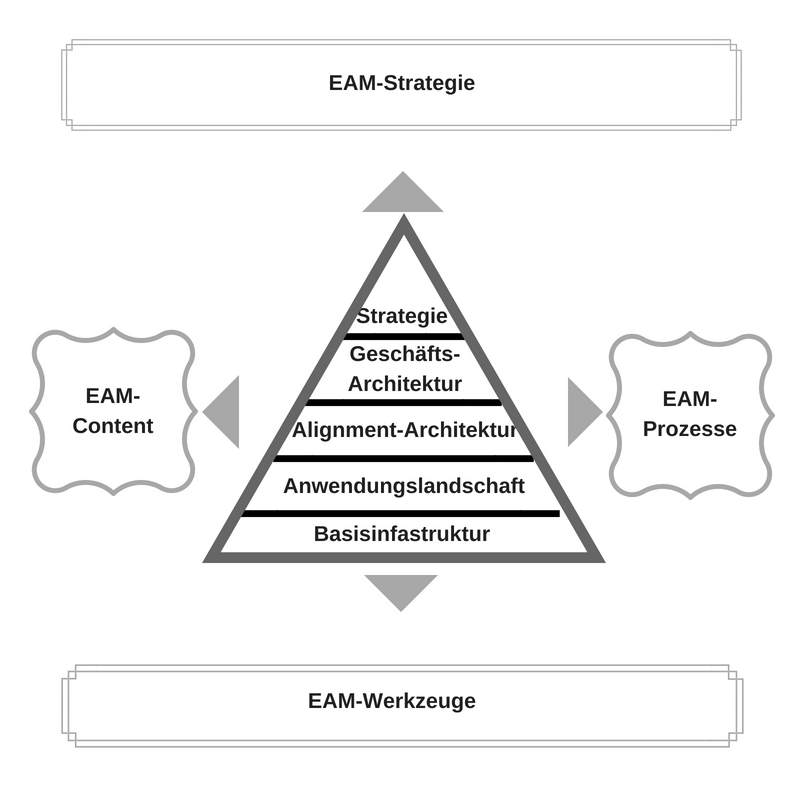
\includegraphics[width=0.75\textwidth]{Abbildungen/Pyramide.png}
\caption{EAM Pyramide und Handlungsfelder (Quelle: \cite{Keuntje2010})}
\label{fig:pyramide}
\end{center}
\end{figure}


Die Organisation der EAM-Pyramide (\autoref{fig:pyramide}) ermöglicht die gesamte Bandbreite der Geschäftsaktivitäten als Ganzes zu sehen. Dies erleichtert das EAM-Team auf bestimmte Ziele konzentrieren und die Verfahren in der  Reihe einer nach dem anderen implementieren damit die nicht ihre Zeit mit vielen  Projekte verlieren, die zeitraubend und anstrengend sind.Die vom Leser gesehene Stratifizierung der Ebenen gliedert sich in die 5 Unterstufen.

\paragraph{Basisinfastruktur} Auf der unteren Ebene befinden sich die IT Architekturelemente einer Firma. Hardwarekomponeneten (Netze,Speicherlösungen) und die Technologiekomponente (Betriebsysteme, Datenbanksysteme) werden durch Technologie Normen standardisieren und skalierbar zu gestalten.

\paragraph{Anwendungslandschaft} Die Anwendungskomponente können über Dienste, Schnittstellen und IT-Werkzeuge die Anwendungen integrieren und nach fachlichen Punkten zu Anwendungsplattformen gruppieren.

\paragraph{Alignment-Architektur} Die mittlere Ebene der Pyramide bildet die Verbindung zwischen den Geschäftsarchitektur und Anwendungslandschaft. An diesem Punkt wird der aktuelle Stand den Anwendungen mit den Geschäftsprozessen und Geschäftsfähigkeiten  neu justiert, damit die Geschäftsarchitektur auf die oberste Ebene anpassen kann.

\paragraph{Geschäftsarchitektur} Auf dieser Ebene wird die gesamte Kultur der Organisation und die Besonderheit ihrer Funktion beschrieben (Standort, Leistungen, Produkte, Dienste, Organisation).Diese helfen bei der Entwicklung eines Architekturmodells und der Unterstützung der Bebauungsplanung.

\paragraph{Strategie} Auf der oberste Ebene wird die Unterstützung von Geschäftsmodellen durch technologische Leistengen gelingen, um eine zusammenhängende erfolgreiche Geschäftsstrategie zu erreichen, die die unteren Ebenen der Pyramide steuern kann.
\mbox{}\\

Die Pyramide ist das Herzstück der Tätigkeit von EAM, aber um die Architektur wertschätzen zu können, müssen die Felder in Kontakt mit ihr bleiben. Jeder von ihnen trägt unterschiedlich zur Gründung von EAM bei und ist verantwortlich für verschiedene Arbeiten.

%%%

\paragraph{EAM Strategie}
basiert auf der Festlegung von Zielen, Kosten, Nutzen und dem reibungslosen Ablauf von EAM. Als ersten Schritt im Integrationsprozess leiten die Architekten die Erstellung eines EAM-Teams, um den Fortschritt des Projekts zu überwachen und anzupassen und dann empfehlen sie die Bestimmung von 4 Paketen:
%%%%%%

\textbf{EAM Maturity Check}
Hier wurde die bereits vorhandenen Unternehmensarchitektur, die Art ihrer Verwaltung und die existierenden Elemente, der IT Manager helfen, die Unternehmenskultur zu verstehen und die Ist-Zustand zu bestimmen. Die Erstellung eines Fragebogens wäre sehr hilfreich.

\textbf{EAM Business Case}
Damit Unternehmer Kosten und Nutzen von EAM berechnen können, ist es wünschenswert ein Business Case, die die Nutzenpotenziale und Gewinne dieser Investition erfasst.

\textbf{EAM Ziele und Kennzahlen}
Die Festlegung von strategischen, taktischen und operativen Zielen ist es sehr wichtig um geschäftlichen Anforderungen auszurichten. Durch die Ziele den Nutzen werden einige wesentlichen Kennzahlen zum Messen der Ziellerreichung für EAM anzuordnen.

\textbf{EAM Programm und Roadmap}
An diesem Punkt wird die Formulierung des Einführungsplans gemacht. Also alle Regeln und Aktivitäten, die in den verbleibenden Handlungsfeldern und ihrer Synchronisation folgen werden.
\setlength{\leftskip}{0pt}
%%%

\paragraph{EAM-Content} Mit der Hilfe einem EAM-Werkzeug oder Framework wird ein geeignetes Metamodel entwickelt. Die Modellierungsprinzipien mussten deutlich die Richtlinien den Ebenen der EAM Pyramide betrachten und den Plan für Stufe vorsichtig entwerfen.

\paragraph{EAM-Prozesse} Bei diesem Feld werden manche Schritte gemacht um die Unternehmensarchitektur mit strategische und taktische Planung, nachhaltig steuerbar zu machen. Lösungsszenarien werden entwickelt damit die Beteiligten herausfinden können mit welchen Anwendungen, die geschäftliche Anforderungen umgesetzt werden, um eine optimale Bebauung von Anwendungen zu erreichen (Bebauungsplan).  Nach der Beschaffung des Bebauungsplans folgt seine Übergabe im Bereich IT-Projekt-Portfolio Management damit die finanzielle Kontrolle und Durchführung des Projekts mit der notwendigen finanziellen Zuteilung des Plans verwirklichen kann.

\paragraph{EAM-Werkzeuge}
Die EAM-Tools zentralisieren die verteilte Dokumentation der Unternehmensarchitektur. Es gibt viele Arten von Werkzeugen, aber es ist sehr wichtig, das geeignete Werkzeug für die neue Architektur zu finden. Hier sollte Das Ist-Zustand berücksichtigt werden, damit Anwendungen mit EAM-Tools abgeglichen werden können. Der Schwierigkeitsgrad ist Heutzutage eine Entscheidung über einen modernen und nachhaltigen Werkzeug zu treffen.
\mbox{}\\

Wie aus dem Zusammenhang ersichtlich ist, gibt es eine große Menge an Anpassungsmaßnahmen, die das Unternehmen in die verschiedenen Bereiche des Unternehmens integrieren muss. Viele Arbeitseinsätze müssen geändert werden, die Archive werden diversifiziert, der Alltag der Mitarbeiter wird sich ändern.

\section{Erfolgsfaktoren}
Es ist Zweifelhaft für das Unternehmen manchmal zu schauen ob EAM  einen Wertbeitrag erzeugt. Manche merken dass die Umsetzung fachlicher Anforderungen in Anwendungen länger dauert und teurer ist als zuvor ohne EAM.
Der Erfolg oder Misserfolg jedes Projekts wird nicht nur von direkten Teilnehmern, sondern auch von einer Reihe von externen Akteuren bestimmt. Er  liegt vor allem in einer Vielzahl kritischer unterschiedlicher Faktoren.
\\
\textbf{Schnelle Ergebnisse}: Das Projekt muss das Erreichen kurzfristiger Ziele sicherstellen. Es ist wichtig, das Interesse des Managements am Projekt wach zu halten. Um dies zu erreichen, muss es schnell die notwendigen Ergebnisse für das Unternehmen erzielen. Wenn unmittelbare Ergebnisse nicht innerhalb von 3 Jahren auftreten, wird das Interesse am Projekt deutlich reduziert.
\\
\textbf{Top-Manager}: Sein Hauptzweck ist es, Probleme in der Organisation zu identifizieren und zu beseitigen. CIOs müssen nicht nur Probleme rechtzeitig identifizieren, sondern auch eine klare Vorstellung von den Ansätzen haben, die in jedem konkreten Fall anzuwenden sind.
\\
\textbf{Schrittweises Vorgehen zum Erreichen gesetzter, messbarer Zwischenziele entlang einer definierten Roadmap}: Das Top-Management soll die Richtlinie der Roadmap verfolgen und die Handlungsfelder für EAM Schritt für Schritt durchführen.
\\
\textbf{Taktisches Handeln entlang der Strategie}: Es ist sehr wahrscheinlich wegen der verschiedenen Ziele im Plan (Bugdet, externe Einflussfaktoren, Zwecke von EAM), dass Konflikte zwischen den Mitgliedern des EAM-Team entstehen. Für jede Lösung müssen Nutzen, Zeitpläne, Kosten und Risiken bewertet, und die Bebauungspläne berücksichtigt werden.
\\
\textbf{Begreifen der Unternehmensarchitektur als ein sich evolutionär weiterentwickelndes  Ganzes}: Manchmal läuft die Unternehmensarchitektur nicht so wie geplant, und es gibt zwischen dem Ist-Zustand und dem Soll Zustand einen Unterschied. Ein gute Praxis in einer solchen Situation wäre, wenn die entsprechenden Personen flexible auf diese Fälle reagieren können.
\\
\textbf{Kommunikation zwischen der IT-Organisation und der Business-Organisation mit den Geschäftsbereichen}: Es ist manchmal Zweifelhaft für das Unternehmen zu erkennen, ob EAM nützlich ist und einen Wertbeitrag liefert. Manche merken, dass die Umsetzung fachlicher Anforderungen in Anwendungen länger dauert und teurer ist als zuvor ohne EAM.
\\
\textbf{Kommunikation innerhalb der IT-Organisation}: Die Unternehmensarchitekten , die für zugewiesene Geschäfts- und IT-Domänen das Know-How für die Projekte bereitstellen, sollten die Kommunikation mit dem zentralen EAM-Team vermittelnd betreiben, damit die Projekte richtig durchgeführt werden.\autocite{Krotkov2013}

Die einzelnen Verfahren müssen auf der Grundlage des vorbereitenden Plans durchgeführt werden. Der Manager sollte umgehend auf individuelle Änderungen reagieren und das Team koordinieren, so dass Probleme in der Übergangsphase des Projekts vermieden werden können. Die besten Strategien scheitern nicht, weil sie nicht wachsen können, sondern weil es ist sehr schwierig zu bedienen. Die Aussichten in der Regel an das Managementsystem selbst beschränkt, sondern als wirtschaftliche Realität. Daher ist das Hauptziel der erfolgreichen Verwaltung der Konfigurationsmanager Wunsch nach Selbstverbesserung und Bedingungen für die Schaffung einer kohärenten Gruppe und geistiger Entwicklung ihrer Mitglieder zu schaffen.

Daher sollte eine effiziente Architektur diese oben genannten Trends harmonisch kombinieren. Die Verwendung aller aufgeführten Funktionen führt zu dem gewünschten Ergebnis und hilft, die dem Manager zugewiesenen Probleme und Aufgaben zu lösen. Ein moderner Manager sollte in der Lage sein, das Problem aus verschiedenen Blickwinkeln zu sehen und eine ausgewogene, vielschichtige und ganzheitliche Sicht auf alle zu haben. ,als auch sich zu entwickeln und ihre persönliche Effektivität zu steigern. Die Verwendung von allen registrierten Fähigkeiten (Kompetenzen? durch den Treuhänder wird das gewünschte Ergebnis so schnell wie möglich geben und die Probleme und Aufgaben an den Administrator zugewiesen lösen.


\section{Misserfolgsfaktoren}
Jüngsten Berichten zufolge scheitern 66% der architektonischen Geschäftsinitiativen. Aber warum? In den letzten Jahren gab es viele Diskussionen, Expertenmeinungen und schriftliche Stellungnahmen zu diesem Thema.
Die Geschäftsarchitektur wurde vor ein paar Jahren entwickelt, um der wachsenden Komplexität von IT-Systemen und ihrer schlechten Ausrichtung auf Geschäftsziele gerecht zu werden. Dieselben Probleme bestehen auch heute noch und werden durch den beschleunigten technologischen Wandel verstärkt.
Im Folgenden finden Sie eine Liste, warum viele Enterprise Architecture-Initiativen fehlschlagen.
All dies wird sehr optimistisch beschrieben. Es kann sehr leicht sein, den Fehler zu machen und gegen einige Regeln zu stimmen und die Vorschriften nicht zu berücksichtigen. Der Manager sollte nicht nur die Erfolgsfaktoren kennen, sondern auch die Faktoren des Scheiterns betrachten.
 Es ist sehr nützlich, um die ineinandergreifenden Menschen zu wissen, welche Maßnahmen sollten Sie vermeiden, bevor Sie schnell reagieren kann, wenn Sie feststellen, dass ein Dienst, der ‚eine Entscheidung, die Leitungen genommen wurde das Projekt zu kollabieren.
Der falsche Lead-Architekt: Eine Person kann EA verstehen, hat jedoch ineffiziente Führungsqualitäten, die nicht zu einer guten Organisationsstruktur und Personalstärke beitragen können.
Überwachung und Inflexibilität gegenüber der Unternehmenskultur: Für eine erfolgreiche EA muss die Unternehmenskultur bei der Planung und Gestaltung von EA für die Organisation berücksichtigt werden.
Verspätete Einführung einer effektiven EA-Governance: EA-Governance-Prozesse müssen so früh wie möglich festgelegt werden, statt auf mehr Architekturinhalte zu warten.
Nicht genug Zeit für Kommunikation: Unternehmensarchitekten müssen die Mitarbeiter unterrichten. Es ist effizient, dass Organisationen einen EA-Kommunikationsplan mit Nachrichten entwickeln und ausführen, die auf jede Zielgruppe zugeschnitten sind.
Die Auswirkungen nicht messen und nicht kommunizieren: Der Wert von EA ist oft indirekt, was das EA-Programm dem Risiko des Scheiterns aussetzt. Es wird empfohlen, dass Unternehmensarchitekten eine Präsentation geben, um jede Erfolgsgeschichte von EA, die auf ein Projekt angewendet wird, zu demonstrieren.
Nicht nur Technical Domain-Level-Architektur: EA ist viel breiter, sie umfasst Business-, Informations- und Lösungsarchitektur und nicht nur die technische Domäne. Why Enterprise Architecture fails to deliver benefits to the business Published on February 22, 2016.Oluwaseyi Ojo Ceng. Linkedin Artikel
Mangel an Sponsoring: Gut gesponserte Architekten können Vertrauen aufbauen, indem sie konsistent aussagekräftige Ergebnisse liefern. Ein Mangel an Sponsoring wird sogar die besten Architekten zum Scheitern bringen.
Wartung der EA Artifact Factory: EAM-Teams sollten sich darauf konzentrieren, häufige, aussagekräftige und messbare Geschäftsergebnisse zu erzielen.
An ein bestimmtes Framework oder einem Tool klammern: Es gibt mehr als 80 EA-Frameworks. Der beste Ansatz besteht darin, alle wichtigen Frameworks zu kennen, das meiste von dem, was Sie gelernt haben, zu verwerfen und die verbleibenden 10\% auf eine Weise zu mischen, die der Unternehmenskultur, der Reife und den Geschäftszielen entspricht.
Denken, dass Enterprise Architecture der Technologiearchitektur entspricht: Die meisten EA-Programme werden von der IT initiiert und kommen nie über den Technologiebereich hinaus. Obwohl Technologiestandards, Technologie-Roadmaps und solide technische Verfahren einfachere, billigere, tragbare, wiederverwendbare und besser unterstützbare Lösungen bieten, stimmen sie Ihre IT-Investitionen nicht mit den Geschäftszielen ab und werden Ihr Unternehmen nicht mit technologischen Innovationen versorgen.
Das Wort "Enterprise" wörtlich nehmen: Um Architektur auf die reale Unternehmensebene zu bringen, bedarf es einer ausgereiften und engagierten Organisation. Wenn man versucht, den Unternehmensaspekt zu früh zu weit zu schieben, wird man scheitern.

Die erfolglose Umsetzung von Entscheidungen, ihre unnötige Arbeit oder Inkongruenz mit den am Arbeitsplatz gesetzten Zielen wirkt sich unmittelbar auf andere Ebenen aus. Beispielsweise kann eine falsch entworfene Anwendung die organisatorische Leistung beeinträchtigen. Dies wiederum kann den Gewinn aus den Dienstleistungen für die Kunden reduzieren.
Das Problem wird durch die Tatsache verstärkt, dass diese negativen Effekte schwer zu bestimmen sind, wenn die Messung der Erfolgskriterien nur schlecht oder nicht koordiniert zwischen den Ebenen erfolgt.
Jede Veränderung in einem Geschäft wie im täglichen Leben des Menschen folgt einer Vielzahl von Entscheidungen, die wir treffen.
Um also die Architektur des Unternehmens erfolgreich zu verändern, müssen wir berücksichtigen, was genau geändert werden muss, wann es geändert werden muss und wen es ändern wird.
Das Erzielen einer effizienten EAM ist eines der wichtigsten Geschäftsziele. Viele Unternehmen haben von seiner Konsolidierung profitiert. Wie weiter erhöht den Bedarf an den technischen Fortschritt und die Entwicklung neuer Anwendungen, Programme, fühlen sich mehr Unternehmen Systeme, die die Voraussetzung für die Gestaltung einer solchen Architektur.
Im Anschluss an den technologischen Fortschritten ist es selbstverständlich, dass nicht nur der private Sektor oder ein bestimmte Partner in einer Wirtschaft schrittweise zu entwickeln. Der Fortschritt eines Landes hängt von der Regierung, ihrem Bildungssystem und ihrem gesunden Bankensystem ab.
Deshalb, um diesen technologischen Fortschritt in einem Land zu halten und gedeihen transparent (etwas, das viele Länder wünschen), die Verwirklichung Architektur zu erleichtern und Bürokratie reduzieren sollte und andere Wirtschaftsbereiche mit einer technologischen Architektur auszurichten.

In den folgenden Kapiteln werden die Vorteile der EAM in einer Bank betrachten und wird am Beispiel der BIAN, die Regierungs EA der Regierung von Dänemark und den Niederlanden und dem Experiment von Norwegen für die Einrichtung von EA für Universitäten zitieren.


\chapter{Fallbeispiele}
% 1800 Wörter
\section{EA im Bankensektor}
\subsection{EAM Banken}
\subsection{BIAN}
\section{EA in Regierungen}
\subsection{EA in Regierungen}
\subsection{NEA (NL, DK)}
\section{EA im Bildungssektor}
\subsection{EA im Bildungssektor}
\subsection{EA im tertiären Bildungsbereich (NO)}

\chapter{Fazit}
% 400 Wörter / 1S
% Ein Satz?
\begin{itemize}
\item EAM findet sich hauptsächlich in großen Unternehmen.
\item Mit der Einbindung von EAM können sowohl in Entscheidungsprozessen als auch in den Routineaufgaben ganz natürliche Veränderungen erreicht werden.
\item Ein CIO sollte die richtigen Leute auswählen, um ein Team zu gründen.
\item Die Geschäftsarchitektur der Bank kann helfen, verschiedene Bankverwaltungssysteme aufzubauen.
\item BIAN Framework bietet eine gute Architektur, aber es ist teuer und die Unternehmen müssen ihre Unternehmen unterstützen.
\item Die Anwendung der EA könnte die Qualität öffentlicher Dienste verbessern. \item Die NEA von Dänemark basiert auf den einzelnen Planungsprozessen, aber die Niederländische NEA besteht aus einer Reihe von Prinzipien und Richtlinien.
\item Die Einführung einer EA im Bildungssystem ist schwierig. Die Befragten in Norwegen antworteten, dass es keine Bereitschaft gibt, sowohl in der Geschäftsleitung als auch auf organisatorischer Ebene.
\item Im Vergleich dazu ist es einfacher, EA im privaten Sektor (Unternehmen, Banken) anstatt im öffentlichen Sektor (Bildung und Regierung) zu integrieren.
\end{itemize}
% Ein Satz?

\printbibliography

\end{document}  